% Appendix A

\chapter{Manual de usuario} % Main appendix title

\label{AppendixA} % For referencing this appendix elsewhere, use \ref{AppendixA}


\section{Descripción}
El medidor (nombre) es un dispositivo capaz de medir tensión y voltaje de línea y realizar cálculos de potencia activa y reactiva, como mediciones de fase. El dispositivo

\section{Características generales}

\begin{itemize}
\item Alimentación de 8 a 28V (AC).
\item Consumo menor a 5700W.
\item Puerto de comunicación serial RS232/Rs485.
\item Menú serie para configuración en boot.
\item Leds de referencia.
\item Capacidad de mediciones alterna para  2200V o 380V.
\end{itemize}


\section{Instalación}

\subsection{Instalación mecánica}

El equipo está diseñado para montaje sobre riel DIN. Se calza sobre riel. EN sus laterales se encuentra una etiqueta con descripción de borneras para el conexionado.


\begin{figure}[!htb]
	\centering
	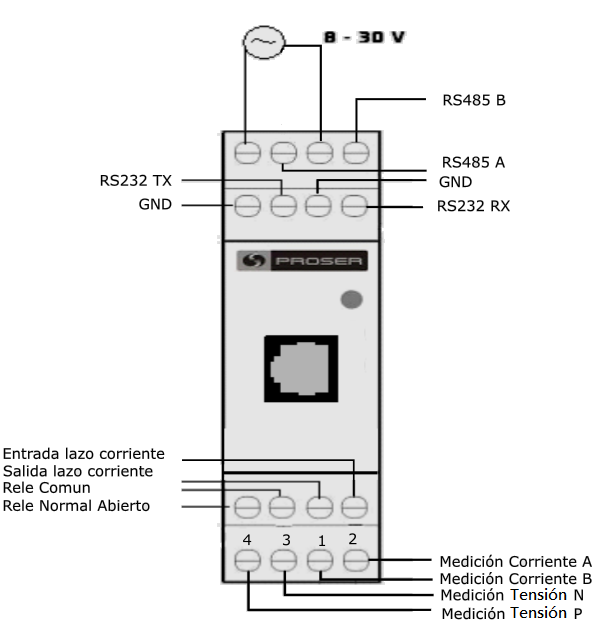
\includegraphics[width=\textwidth , keepaspectratio]{Figures/ApendixA/conectores2.png}
	%\caption{}
	\label{fig:ADEfuncbloc}
\end{figure}

\subsection{Instalación eléctrica }
El equipo se alimenta con tensión continua de un rango de 8 a 40 voltios.
A continuación se detalla la tabla de conexionado:
% Please add the following required packages to your document preamble:
% \usepackage{booktabs}
\begin{table}[!htb]
\begin{tabular}{@{}lll@{}}
\toprule
Borne & REF         & Descripción                \\ \midrule
1     & CloopIO     & Salida lazo corriente 4 20 \\
2     & CloopV      & Entrada 4 20               \\
3     &             & Comun de rele              \\
4     &             & Normal abierto relé        \\
5     & AC          & Entrada alterna medidor    \\
6     & AC          & Entrada alterna medidor    \\
7     & B           & B RS485                    \\
8     & A           & A RS485                    \\
9     & GND digital &                            \\
10    & GND digital &                            \\
11    & RS232 Rx    &                            \\
12    & RS232 Tx    &                            \\
13    & Shunt N     & Medición corriente         \\
14    & Shunt P     & Medición corriente         \\
15    & Voltaje N   & Medición tensión           \\
16    & Voltaje P   & Medición tensión           \\ \bottomrule
\end{tabular}
\end{table}


\subsection{Entradas discretas}

\subsection{Entradas analógicas}

\subsection{Salidas discretas}
El medidor viene provisto de una salida discreta del tipo open collector que puede manejar una carga con una corriente máxima de hasta 100mA.

\subsection{Puerto Serial}
El medidor viene provisto de un puerto de comunicaciones serial que permite conectarse a cualquier dispositivo con puerto RS232 o RS485 .
La velocidad de comunicación  está fijada a 9600bps. Además el puerto se comunica en protocolo Modbus seleccionable de RTU o ASCII con paridad elegible.

\section{Operación}

\subsection{Indicador luminosos LED}

El medidor cuenta con dos indicadores luminosos LED . Un LED indica para la calibración dependiente de la constante de calibración y otro Para indicar el estado del sistema.


El LED del equipo indica:

\begin{itemize}
\item Led (verde) encendido : Corriendo menú serie
\item Led (rojo) encendido: Esperando 10 segundos a menú serie
\item Led (verde) titilante  a 500 ms : Corriendo programa de lectura
\item Led (rojo) titilante  a 500 ms : Puerto 232
\item Led (rojo) apagado : Puerto 485
\item CF2 (Led Q1)  Es proporcional a la potencia activa.
\end{itemize}


\subsection{Configuración}
El medidor tiene embebido un menú, que permite configurar el equipo y realizar pruebas de funcionamiento por medio de un terminal estándar (ej: Hyperterminal de Windows).

Esto permite acceder a la configuración del equipo sin necesidad de un software adicional.

El ingreso al menú de configuración se realiza conectando un terminal configurado en 9600 8N1.


\subsubsection{Menú principal}
En el menú de configuración principal se puede apreciar las opciones de ajuste del equipo.

\textcolor{orange}{
PROSER MEI-380V, S/N: SV-0500003}

\definecolor{mygreen}{RGB}{40, 100, 60}

\textcolor{mygreen}{MenuPrincipal}

\textcolor{blue}{1: Visualización variables.}

\textcolor{blue}{2: Puerto serie.}

\textcolor{blue}{3: Salida 4-20mA.}

\textcolor{blue}{4: Alarma.}

\textcolor{blue}{D: Aplicar valores por defecto globalmente.}

\textcolor{blue}{G: Guarda configuración.}

\textcolor{blue}{ESC: Abandonar terminal.}



Descripción de las Opciones:


\textcolor{blue}{1-2 .}
Ingresando la opción 1 a 4 se accede a las distintas opciones del equipo.

\textcolor{blue}{D .}
Modifica todos los valores a los predeterminados.

\textcolor{blue}{G .}
Guarda la configuración seteada y aplica los cambios.

\textcolor{blue}{ESC.}
Abandona la terminal, esta se cierra hasta que se reinicie el dispositivo.

\subsubsection{OPCIÓN 1: Visualización de variables}
Esta opción permite visualizar las variables que se encuentra recopilando el sensor.

\textcolor{mygreen}{VISUALIZACIÓN DE VARIABLES }

\textcolor{blue}{Tensión (V)}

\textcolor{blue}{Corriente (A)}

\textcolor{blue}{Potencia Activa (W)}

\textcolor{blue}{Potencia Reactiva (W)}

\textcolor{blue}{Frecuencia (Hz)}

\textcolor{blue}{Factor de potencia}

\textcolor{blue}{Totalizado (Kw/h)}

\textcolor{blue}{ESC: Menú principal.}



Descripción de las Opciones

\textcolor{blue}{ESC.}
Abandona este menú, vuelve al menú principal.

\subsubsection{OPCIÓN 2: Puerto serie}

Esta opción configura el puerto serie por lo que se recomienda re-configurar el puerto de comunicación que se esté utilizando al cambiar alguna variable. Esta opción también configura parámetros del protocolo Modbus.

\textcolor{mygreen}{CONFIGURACION PUERTO SERIE}

\textcolor{blue}{1* CONFIGURACION PUERTO SERIE * [Valores predeterminados]}

\textcolor{blue}{1: Baud rate: 9600}

\textcolor{blue}{2: Bits de datos: 8 Bits}

\textcolor{blue}{3: Paridad: NINGUNA}

\textcolor{blue}{4: Bits de parada: 1}

\textcolor{blue}{5: Dirección MODBUS: 5}

\textcolor{blue}{6: Protocolo modo: RTU}

\textcolor{blue}{7: Protocolo tipo: ENRON}

\textcolor{blue}{8: Tipo de puerto: RS485}

\textcolor{blue}{D: Aplica configuración por defecto.}

\textcolor{blue}{ESC: Menú principal.}



Descripción de las Opciones

\textcolor{blue}{1.Baud rate }	
Permite ajustar el Baud Rate del puerto.

\textcolor{blue}{2.Bits de datos}
Ajusta los bits de datos entre 7 u 8 bits.

\textcolor{blue}{3.Paridad}
Ajusta la paridad entre par o impar.

\textcolor{blue}{4.Parada}
Ajusta los bits de parada, puede ser 1 o 2.

\textcolor{blue}{5.Dirección Slave del Modbus}
Setea la dirección de esclavo que tendrá el dispositivo para el protocolo Modbus.

\textcolor{blue}{6.Modo del Protocolo}
Tipo de protocolo MODBUS, puede ser ASCII o RTU.

\textcolor{blue}{8.Tipo de puerto}
Selecciona entre los dos posibles puertos de salida, RS232 o RS485.


\subsubsection{OPCIÓN 3: Salida 4-20mA}
\textcolor{mygreen}{SALIDA ANALOGICA 4-20mA}

\textcolor{blue}{Cambiar variable: Seleccione una opción (1-6)}

\textcolor{blue}{1 - Tensión.}

\textcolor{blue}{2 - Corriente.}

\textcolor{blue}{3 - Potencia Activa.}

\textcolor{blue}{4 - Potencia Reactiva.}

\textcolor{blue}{5 - Frecuencia.}

\textcolor{blue}{6 - Factor de potencia.}

\textcolor{blue}{D: Aplica configuración por defecto.}

\textcolor{blue}{ESC: Menú principal.}


 

Opciones disponibles

\textcolor{blue}{1-6 .}
De estas opciones se elige una variable que se encuentra midiendo el dispositivo. La salida de enlace de corriente es proporcional a la variable elegida.

\textcolor{blue}{D .}
Modifica los valores a los predeterminados.

\textcolor{blue}{ESC.}
Abandona este menú, vuelve al menú principal.

\subsubsection{OPCIÓN 4: Alarma}

Esta opción permite definir qué variable medida será la utilizada para accionar el relé interno y cómo lo accionara.

\textcolor{mygreen}{ALARMA}

\textcolor{blue}{S: Salida a Relé: INACTIVA}

\textcolor{blue}{L1: Límite mínimo para activación: 100}

\textcolor{blue}{L2: Límite máximo para des-activación: 105}

\textcolor{blue}{Cambiar variable: Seleccione una opción (1-6)}

\textcolor{blue}{1 - Tensión.}

\textcolor{blue}{2 - Corriente.}

\textcolor{blue}{3 - Potencia Activa.}

\textcolor{blue}{4 - Potencia Reactiva.}

\textcolor{blue}{5 - Frecuencia.}

\textcolor{blue}{6 - Factor de potencia.}

\textcolor{blue}{Variable asociada: “ ”}

\textcolor{blue}{D: Aplica configuración por defecto.}

\textcolor{blue}{ESC: Menú principal.}

Opciones disponibles


\textcolor{blue}{1-6.}
De estas opciones se elige una variable que se encuentra midiendo el dispositivo. La alarma se activa una vez que el valor de la variable supera el límite de activación.

\textcolor{blue}{D.}
Modifica los valores a los predeterminados.

\textcolor{blue}{ESC.}
Abandona este menú, vuelve al menú principal.




\subsection{TABLA DE REGISTROS MODBUS}

Los registros son solo lectura, en el caso de solicitar un registro que no se encuentre en la tabla se recibirá una excepción.

\begin{table}[h]
%\caption[Registros modbus en software]{Registros generados para la comunicación modbus.}
\begin{tabular}{@{}lllll@{}}
\toprule
\begin{tabular}[c]{@{}l@{}}Dirección \\ del \\ Registro\end{tabular} & \begin{tabular}[c]{@{}l@{}}Número \\ del\\ parámetro\end{tabular} & Descripción                    & Unidades & Tipo de dato \\ \midrule
7001                                                                 & 1                                                                 & Voltaje Instantaneo            & Volts    & Float 32     \\
7003                                                                 & 2                                                                 & Voltaje rms                    & Volts    & Float 32     \\
7005                                                                 & 3                                                                 & Corriente instantánea          & Ampere   & Float 32     \\
7007                                                                 & 4                                                                 & Corriente rms                  & Ampere   & Float 32     \\
7009                                                                 & 5                                                                 & Potencia activa                & Watt     & Float 32     \\
7011                                                                 & 6                                                                 & Potencia reactiva              & VA       & Float 32     \\
7013                                                                 & 7                                                                 & Factor de potencia             & -        & Float 32     \\
7015                                                                 & 8                                                                 & Frecuencia                     & Hz       & Float 32     \\
7017                                                                 & 9                                                                 & Energía reactiva medida        & Joules   & Float 32     \\
7019                                                                 & 10                                                                & Energía activa Total acumulada & kWh      & Float 32    
\end{tabular}
\label{apendixsmodbs}
\end{table}


\subsection{Menú Calibración}
En el menú de configuración principal se puede apreciar las opciones de ajuste del equipo.  
Menú Principal
1: Visualizador de variables
2: Editor de resistencias en uso
3: Editor de registros de ganancia
4: Editor de registros de calibración
5. Editor de salida 4 -20 mA
D: Aplicar valores por defecto globalmente.
G: Guarda configuración.
ESC: Abandonar terminal.

\subsubsection{OPCIÓN 2: Editor de resistencias en uso.}

En esta opción se especifican las resistencias soldadas en el circuito electrónico. Las resistencias que se modifican son las utilizadas para los cálculos de medición.


\textcolor{blue}{2: Editor de resistencias en uso}

Resistores de VP - VN (ohms)

Resistor Shunt (ohms)


\subsubsection{OPCIÓN 3: Editor de registros de ganancia.}
\textcolor{blue}{ Editor de registros de ganancia}

\textcolor{blue}{1 Elija ganancia para PGA\_ IA}

\textcolor{blue}{2 Elija ganancia para PGA\_ V}

Opciones

\textcolor{blue}{1. Ganancia 1  = Fondo de escala 500   mV}

\textcolor{blue}{2. Ganancia 2  = Fondo de escala 250   mV}

\textcolor{blue}{3. Ganancia 4  = Fondo de escala 125   mV}

\textcolor{blue}{4. Ganancia 8  = Fondo de escala 62.5  mV}

\textcolor{blue}{5. Ganancia 16 = Fondo de escala 31.25 mV}

\textcolor{blue}{6. Ganancia 22 = Fondo de escala 22.7  mV}

\subsubsection{OPCIÓN 4: Menú - Calibración de variables:}

Menú - Calibración de variables:

Calibrar Voltaje
\begin{enumerate}
\item Ingreso: Ingrese el voltaje que se está midiendo (cercano al nominal)
\item Se realizan los cálculos
\end{enumerate}

Se ingresa un voltaje cercano al nominal y se realiza el siguiente cálculo

\begin{figure}[!htb]
	\centering
	
\includegraphics[width=\textwidth , keepaspectratio]{Figures/ApendixA/ec1.png}
	%\caption{}
	\label{fig:ecu1A}
\end{figure}

El resultado se guarda en el registro AVGAIN 


\begin{enumerate}
\setcounter{enumi}{2}
\item Ingreso: Ingrese el voltaje que se está midiendo (menor al 10\% del nominal)
\item Se realizan los cálculos
\end{enumerate}

Se ingresa un voltaje menor al 10\% del nominal y se realiza el siguiente cálculo:

\begin{figure}[!htb]
	\centering
	
\includegraphics[width=\textwidth , keepaspectratio]{Figures/ApendixA/ec2.png}
	%\caption{}
	\label{fig:ecu2A}
\end{figure}

El resultado se guarda en el registro VRMSOS

\begin{enumerate}
\setcounter{enumi}{4}
\item Se muestra el resultado
\end{enumerate}



Calibrar Corriente

\begin{enumerate}
\item Ingreso: Ingrese la corriente que se está midiendo (cercano al nominal)
\item Se realizan los cálculos
\end{enumerate}

\begin{figure}[!htb]
	\centering
	
\includegraphics[width=\textwidth , keepaspectratio]{Figures/ApendixA/ec3.png}
	%\caption{}
	\label{fig:ecu3A}
\end{figure}

\begin{enumerate}
\setcounter{enumi}{2}
\item Ingreso: Ingrese la corriente que se está midiendo (menor al 10% del nominal)
\item Se realizan los cálculos
\end{enumerate}
\begin{figure}[!htb]
	\centering
	
\includegraphics[width=\textwidth , keepaspectratio]{Figures/ApendixA/ec4.png}
	%\caption{}
	\label{fig:ecu4A}
\end{figure}

\begin{enumerate}
\setcounter{enumi}{4}
\item Se muestra el resultado
\end{enumerate}

Calibrar Potencia
\begin{enumerate}
\item Ingreso:Se ingresa el valor de la potencia que se está midiendo
\item Se realizan los cálculos
\end{enumerate}

\begin{figure}[!htb]
	\centering
	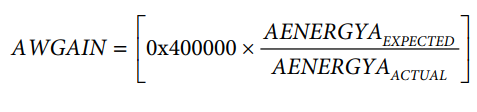
\includegraphics[width=\textwidth , keepaspectratio]{Figures/ApendixA/ec5.png}
	%\caption{}
	\label{fig:ecu5A}
\end{figure}

\begin{enumerate}
\setcounter{enumi}{2}
\item Se muestra el resultado
\end{enumerate}

\subsubsection{OPCIÓN 5: Editor de registros de ganancia}
Menu - Calibración de salida 4-20 mA:
La salida actualmente es dependiente de la variable : “(Se muestra la variable dependiente) ”
Se realizaran 3 mediciones

\begin{itemize}
\item Se inserta el valor mínimo pretendido para 4mA a la placa, se pide que se \item ingrese el valor por consola.
\item Se realizan cálculos.
\item Se Inserta el valor máximo de la variable pretendida para 20mA a la placa, se pide que se ingrese el valor por consola.
\item Se realizan cálculos.
\item Se pide que se inserte un valor intermedio y se pide que ingrese el valor por consola
\item Se calibra y sale del menú

\end{itemize}

%%%%%%%%%%%%%%%%%%%%%%
%%%%%%%%%%%%%%%%%%%%%%%
%%%%%%%%%%%%%%%%%%%%%%%%%

\section{Características técnicas}
Montaje
\begin{itemize}
\item Riel DIN
\end{itemize}
Alimentación
\begin{itemize}
\item 8 a 30 VCC
\item Consumo <0.7W
\end{itemize}
Puertos de comunicación
\begin{itemize}
\item RS232 y RS485 (ambos en el mismo puerto)
\item Bbps: 9600
\item Bits: 8
\item Paridad: Sin paridad.
\item En modo Modbus : RTU/ASCII , Par/ Impar/ Sin paridad.
\end{itemize}
Configuración
\begin{itemize}
\item Menú serie embebido
\end{itemize}
Módulo de medición de potencia
\begin{itemize}
\item Precisión con tolerancia de 1%
\item Registros de medición de potencia reactiva y energía.
\end{itemize}
Entradas /Salidas
\begin{itemize}
\item Una salida de comunicación serie
\item 4 entradas analógicas (2 para medcion de voltaje y 2 para medición de amperaje)
\item 1 salida analógica (4-20MA)
\end{itemize}




\section{Medidas y dimensiones}
\begin{figure}[!htb]
	\centering
	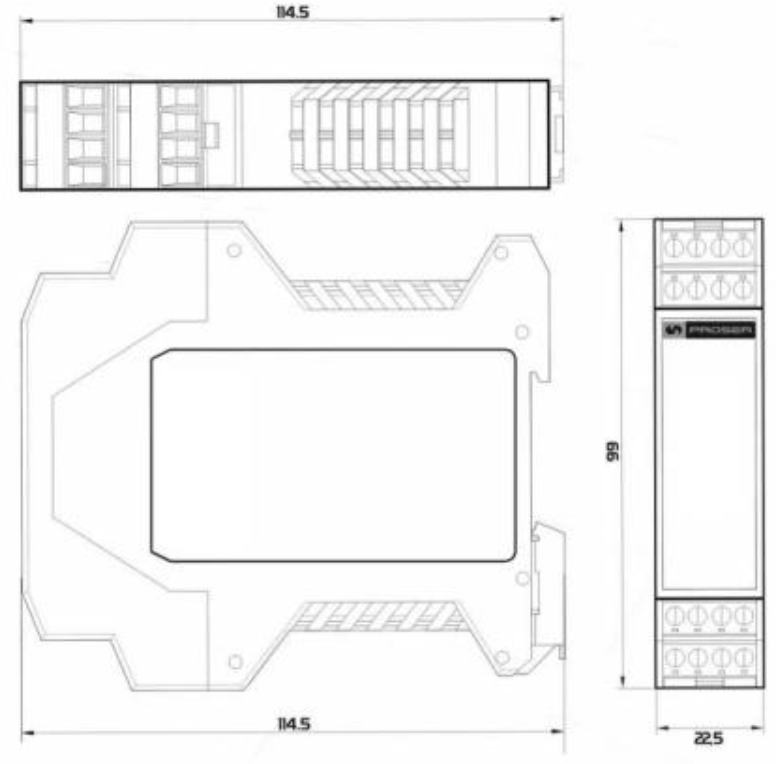
\includegraphics[width=\textwidth , keepaspectratio]{Figures/ApendixA/medidas.png}
	%\caption{}
	\label{fig:ADEfuncbloc}
\end{figure}

Los valores se encuentran en mm  (milímetros).